\documentclass{beamer}

%\usetheme{CambridgeUS}         % tema
% \usecolortheme{orchid}      % cores
\usetheme{metropolis}
\metroset{numbering=fraction, sectionpage=none, subsectionpage=progressbar}
\usecolortheme{seahorse}
\usecolortheme{rose}
\usefonttheme[onlysmall]{structurebold}
\usefonttheme[onlymath]{serif} % fonte modo matematico

\usepackage{framed}
\usepackage{disciplina}
\usepackage{tikz}
\usetikzlibrary{calc,shapes.multipart,chains,arrows}
\usepgflibrary{shapes.multipart}
\newcommand{\eq}{=}

\author[João Araujo Ribeiro]{João Araujo Ribeiro \\ \texttt{jaraujo@uerj.br}}
\institute[UERJ]{Universidade do Estado do Rio de Janeiro} % opcional
\date[EstrInf]{Departamento de Engenharia de Sistemas e Computação}
\pgfdeclareimage[height=0.7cm]{imagens//logo.png}{imagens//logodesc.png}
\logo{\pgfuseimage{imagens//logo.png}}
% Titulo
\title[\sc{Estruturas de Informação I}]{Estruturas de Informação I}
\subtitle{3. Listas baseadas em Listas Encadeadas}

\begin{document}

\begin{frame}
  \titlepage
\end{frame}

\begin{frame}
	\frametitle{Resumo}
	Nesta aula vamos estudar a implementação da interface de lista usando listas encadeadas.
	
	{\footnotesize \texttt{http://www.opendatastructures.org/ods-python/3\_Linked\_Lists.html}}
	\tableofcontents
\end{frame}

\section{3 -  Listas Encadeadas}

\begin{frame}
	\LARGE{\alert{Listas Encadeadas}}
	
	\normalsize
	Nas listas sequenciais anteriores é necessário um grande esforço computacional para operações de inserção e remoção de nós.
	
	Uma forma de permitir o crescimento dinâmico do comprimento máximo de uma  lista é representar a lista por \textit{encadeamento}, onde  os nós são ligados entre si para indicar a relação de ordem entre eles.

\end{frame}

\begin{frame}
\frametitle{Encadeamento}
Cada nó deve conter não apenas o dado mas também a indicação do nó seguinte, casa haja algum. Neste caso, o encadeamento é lógico.

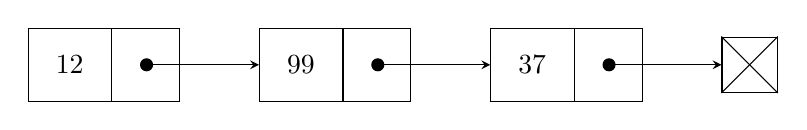
\begin{tikzpicture}[list/.style={rectangle split, rectangle split parts=2,
	draw, rectangle split horizontal}, >=stealth, start chain,inner sep=10pt]

\node[list,on chain] (A) {12};
\node[list,on chain] (B) {99};
\node[list,on chain] (C) {37};
\node[on chain,draw] (D) {};
\draw (D.north east) -- (D.south west);
\draw (D.north west) -- (D.south east);
\draw[*->] let \p1 = (A.two), \p2 = (A.center) in (\x1,\y2) -- (B);
\draw[*->] let \p1 = (B.two), \p2 = (B.center) in (\x1,\y2) -- (C);
\draw[*->] let \p1 = (C.two), \p2 = (C.center) in (\x1,\y2) -- (D);
\end{tikzpicture}
\end{frame}

\begin{frame}
\frametitle{Lista Linear}
 A Lista Linear agrupa informações referentes a um conjunto  de  elementos  que,  de  alguma  forma, se relacionam entre si.
\end{frame}




\begin{frame}
\frametitle{Listas Encadeadas}

\begin{itemize}
	\item Em \alert{listas encadeadas}, elementos consecutivos na lista não implicam em elementos consecutivos na representação (a ordem é \alert{lógica}). \pause
	
	\item Na implementação é necessário armazenar separadamente a informação de um elemento da lista, normalmente o \alert{primeiro}.\pause
	
	
	\item Existem duas formas de se representar listas encadeadas, através de array, denominadas \alert{listas estáticas}, ou por ponteiros chamadas \alert{listas dinâmicas}. 
\end{itemize}

\end{frame}

\begin{frame}[fragile]
	\frametitle{Lista Estática}
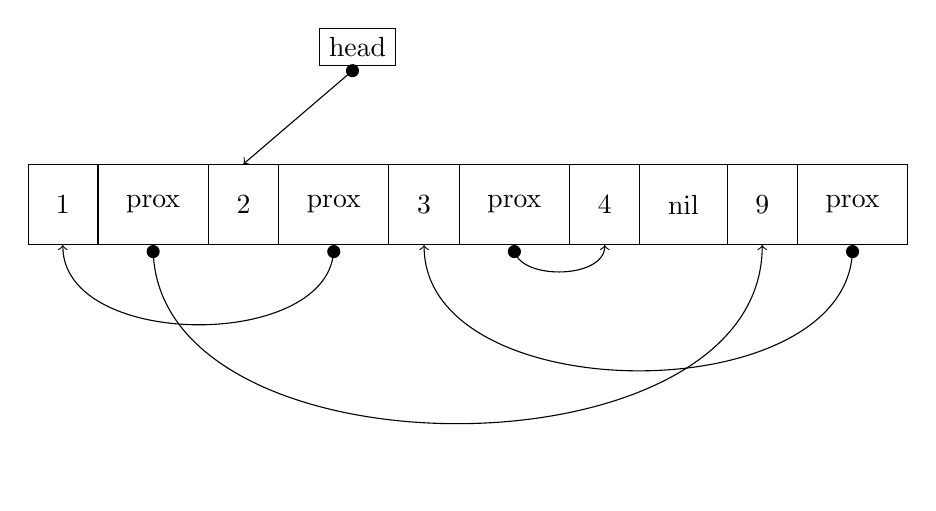
\begin{tikzpicture}[myshape/.style={rectangle split, rectangle split parts=#1, draw, anchor=center,inner sep=10pt}]
\node[draw] at (0.6,4)(head) {head};
\node [myshape=10, rectangle split horizontal] (array) at (2,2)
{1\nodepart{two}prox\nodepart{three}2\nodepart{four}prox\nodepart{five}3
	\nodepart{six}prox\nodepart{seven}4
	\nodepart{eight}nil\nodepart{nine}9\nodepart{ten}prox};

\draw[*->] let \p1 = (head), \p2 = (head.south) in (\x1,\y2) -- (array.three north);
\draw[*->] let \p1 = (array.four south), \p2 = (array.four south) in (\x1,\y2) to[out=-90,in=-90] (array.one south);
\draw[*->] let \p1 = (array.two south), \p2 = (array.two south) in (\x1,\y2) to[out=-90,in=-90] (array.nine south);
\draw[*->] let \p1 = (array.ten south), \p2 = (array.ten south) in (\x1,\y2) to[out=-90,in=-90] (array.five south);
\draw[*->] let \p1 = (array.six south), \p2 = (array.six south) in (\x1,\y2) to[out=-90,in=-90] (array.seven south);

\end{tikzpicture}
\end{frame}

\begin{frame}
	\frametitle{Lista Dinâmica}
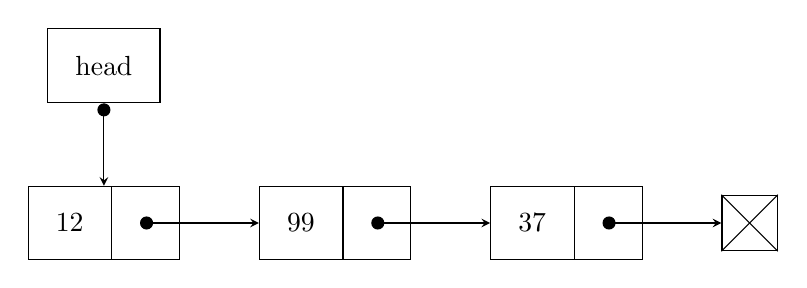
\begin{tikzpicture}[list/.style={rectangle split, rectangle split parts=2,
	draw, rectangle split horizontal}, >=stealth, start chain,inner sep=10pt]

\node[draw] at (0,2)(head) {head};

\node[list,on chain] (A) {12};
\node[list,on chain] (B) {99};
\node[list,on chain] (C) {37};
\node[on chain,draw] (D) {};
\draw (D.north east) -- (D.south west);
\draw (D.north west) -- (D.south east);
\draw[*->] let \p1 = (A.two), \p2 = (A.center) in (\x1,\y2) -- (B);
\draw[*->] let \p1 = (B.two), \p2 = (B.center) in (\x1,\y2) -- (C);
\draw[*->] let \p1 = (C.two), \p2 = (C.center) in (\x1,\y2) -- (D);
\draw[*->] let \p1 = (head), \p2 = (head.south) in (\x1,\y2) -- (A);
\end{tikzpicture}
\end{frame}


\subsection{3.1 Listas Simplesmente Encadeadas- SLList}
\begin{frame}
\frametitle{Listas Simplesmente Encadeadas - SLList}

Uma $ SLList $  (lista simplesmente encadeada) é uma sequência de \textit{Nó}s. Cada nó  $ u $  armazena um valor de dados  $ u.x $  e uma referência  $ u.next $  para o 
próximo nó na sequência. Para o último nó $ w $ na sequência, $ w.next = null $


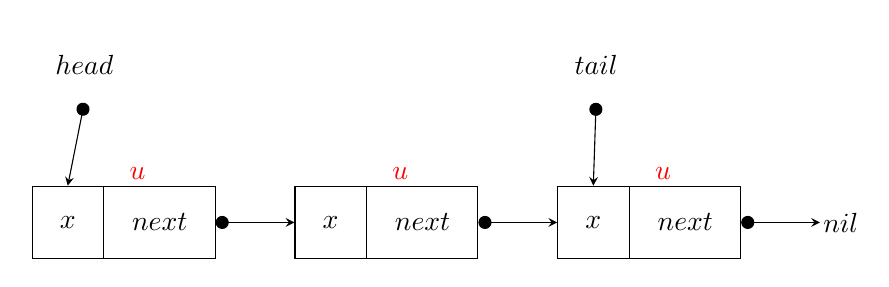
\begin{tikzpicture}[list/.style={rectangle split, rectangle split parts=2,
	draw, rectangle split horizontal}, >=stealth, start chain,inner sep=10pt, every label/.style={red, above right=-4mm}]

\node at (-0.5,2)(head) {$ head $};
\node at (6,2)(tail) {$ tail $};

\node[list,on chain, label=$ u $] (A) {$x$\nodepart{two}$ next $};
%\node at (A.north west) {$ u $};
\node[list,on chain, label=$ u $] (B) {$x$\nodepart{two}$ next $};
\node[list,on chain, label=$ u $] (C) {$x$\nodepart{two}$ next $};
\node[on chain,inner sep=1pt] (D) {$ nil $};
\draw[*->] let \p1 = (A.two east), \p2 = (A.east) in (\x1,\y2) -- (B);
\draw[*->] let \p1 = (B.two east), \p2 = (B.center) in (\x1,\y2) -- (C);
\draw[*->] let \p1 = (C.two east), \p2 = (C.center) in (\x1,\y2) -- (D.west);
\draw[*->] let \p1 = (head), \p2 = (head.south) in (\x1,\y2) -- (A.one north);
\draw[*->] let \p1 = (tail), \p2 = (tail.south) in (\x1,\y2) -- (C.one north);
\end{tikzpicture}
\end{frame}

\begin{frame}
	\frametitle{SLList - initialize}
	
Para eficiência, um $ SLList $ usa as variáveis $ head $ e $ tail $ para 
manter o registro do primeiro e do último nó na sequência, bem como um número 
inteiro $ n $ para acompanhar o tamanho da sequência: 


\begin{framed}
\begin{flushleft}
\hspace*{1em} \ensuremath{\mathrm{initialize}()}\\
\hspace*{1em} \hspace*{1em} \ensuremath{\ensuremath{\mathit{n}} \gets  \ensuremath{0}}\\
\hspace*{1em} \hspace*{1em} \ensuremath{\ensuremath{\mathit{head}} \gets  \ensuremath{nil}}\\
\hspace*{1em} \hspace*{1em} \ensuremath{\ensuremath{\mathit{tail}} \gets  \ensuremath{nil}}\\
\end{flushleft}
\end{framed}
\end{frame}


 \tikzset{
 	invisible/.style={opacity=0,text opacity=0},
 	visible on/.style={alt={#1{}{invisible}}},
 	alt/.code args={<#1>#2#3}{%
 		\alt<#1>{\pgfkeysalso{#2}}{\pgfkeysalso{#3}} % \pgfkeysalso doesn't change the path
 	},
 }
 
\begin{frame}
	\frametitle{Sequência de operações de fila e pilha usando LSE}
	$add(\texttt{x})$
	
	\begin{tikzpicture}[list/.style={rectangle split, rectangle split parts=2, draw, rectangle split horizontal}, >=stealth, start chain,minimum size=6mm]
	\node at (0,-1)(head) {head};
	\node at (8,-1)(tail) {tail};
	
	\node[list,on chain] at(0,-2) (A) {\texttt{a}};
	\node[list,on chain] (B) {\texttt{b}};
	\node[list,on chain] (C) {\texttt{c}};
	\node[list,on chain,draw] (D) {\texttt{d}};
	\node[list,on chain,draw] (E) {\texttt{e}};
	
	\draw[*->] let \p1 = (A.two), \p2 = (A.center) in (\x1,\y2) -- (B);
	\draw[*->] let \p1 = (B.two), \p2 = (B.center) in (\x1,\y2) -- (C);
	\draw[*->] let \p1 = (C.two), \p2 = (C.center) in (\x1,\y2) -- (D);
	\draw[*->] let \p1 = (D.two), \p2 = (D.center) in (\x1,\y2) -- (E);
	\draw[*->] let \p1 = (head), \p2 = (head.south) in (\x1,\y2) -- (A);
	\draw[visible on=<1>,*->] let \p1 = (tail), \p2 = (tail.south) in (\x1,\y2) -- (E);
	
	\node[visible on=<2->,list,on chain,draw] (X) {x\nodepart{two}\alert{$ nil $}};
	\draw[visible on=<2->,*->] let \p1 = (E.two), \p2 = (E.center) in (\x1,\y2) -- (X);
	\draw[visible on=<2->,*->] let \p1 = (tail), \p2 = (tail.south) in (\x1,\y2) -- (X);
	\end{tikzpicture}
	
\end{frame}


\begin{frame}
\frametitle{Sequência de operações de fila e pilha usando LSE}
 		$remove()$
 		
 		\begin{tikzpicture}[list/.style={rectangle split, rectangle split parts=2, draw, rectangle split horizontal}, >=stealth, start chain,minimum size=6mm]
	\node at (0,-1)(head) {head};
	\node at (8,-1)(tail) {tail};
		\node[visible on=<1>,list,on chain] at(0,-2) (A) {\texttt{a}};
		\node[list,on chain] (B) {\texttt{b}};
		\node[list,on chain] (C) {\texttt{c}};
		\node[list,on chain,draw] (D) {\texttt{d}};
		\node[list,on chain,draw] (E) {\texttt{e}};
		\draw[visible on=<1>,*->] let \p1 = (A.two), \p2 = (A.center) in (\x1,\y2) -- (B);
		\draw[*->] let \p1 = (B.two), \p2 = (B.center) in (\x1,\y2) -- (C);
		\draw[*->] let \p1 = (C.two), \p2 = (C.center) in (\x1,\y2) -- (D);
		\draw[*->] let \p1 = (D.two), \p2 = (D.center) in (\x1,\y2) -- (E);
		\draw[visible on=<1>,*->] let \p1 = (head), \p2 = (head.south) in (\x1,\y2) -- (A);
		\draw[visible on=<2->,*->] let \p1 = (head), \p2 = (head.south) in (\x1,\y2) -- (B);
		
		\node[list,on chain,draw] (X) {x\nodepart{two}\alert{$ nil $}};
		\draw[*->] let \p1 = (E.two), \p2 = (E.center) in (\x1,\y2) -- (X);
		\draw[*->] let \p1 = (tail), \p2 = (tail.south) in (\x1,\y2) -- (X);
 		\end{tikzpicture}

\end{frame}

\begin{frame}
	\frametitle{Sequência de operações de fila e pilha usando LSE}
	$pop()$
	
	\begin{tikzpicture}[list/.style={rectangle split, rectangle split parts=2, draw, rectangle split horizontal}, >=stealth, start chain,minimum size=6mm]
	\node at (0,-1)(head) {head};
	\node at (8,-1)(tail) {tail};
	\node[invisible,list,on chain] at(0,-2) (A) {\texttt{a}};
	\node[visible on=<1>,list,on chain] (B) {\texttt{b}};
	\node[list,on chain] (C) {\texttt{c}};
	\node[list,on chain,draw] (D) {\texttt{d}};
	\node[list,on chain,draw] (E) {\texttt{e}};

	\draw[visible on=<1>,*->] let \p1 = (B.two), \p2 = (B.center) in (\x1,\y2) -- (C);
	\draw[*->] let \p1 = (C.two), \p2 = (C.center) in (\x1,\y2) -- (D);
	\draw[*->] let \p1 = (D.two), \p2 = (D.center) in (\x1,\y2) -- (E);

	\draw[visible on=<1>,*->] let \p1 = (head), \p2 = (head.south) in (\x1,\y2) -- (B);
	\draw[visible on=<2->,*->] let \p1 = (head), \p2 = (head.south) in (\x1,\y2) -- (C);
	
	\node[list,on chain,draw] (X) {x\nodepart{two}\alert{$ nil $}};
	\draw[*->] let \p1 = (E.two), \p2 = (E.center) in (\x1,\y2) -- (X);
	\draw[*->] let \p1 = (tail), \p2 = (tail.south) in (\x1,\y2) -- (X);
	\end{tikzpicture}
	
\end{frame}

\begin{frame}
	\frametitle{Sequência de operações de fila e pilha usando LSE}
	$push(\texttt{y})$
	
	\begin{tikzpicture}[list/.style={rectangle split, rectangle split parts=2, draw, rectangle split horizontal}, >=stealth, start chain,minimum size=6mm]
	\node at (0,-1)(head) {head};
	\node at (8,-1)(tail) {tail};
	\node[invisible,list,on chain] at(0,-2) (A) {a};
	\node[visible on=<2->,list,on chain] (Y) {\texttt{y}};
	\node[list,on chain] (C) {c};
	\node[list,on chain,draw] (D) {d};
	\node[list,on chain,draw] (E) {e};
	
	\draw[visible on=<2->,*->] let \p1 = (Y.two), \p2 = (Y.center) in (\x1,\y2) -- (C);
	\draw[*->] let \p1 = (C.two), \p2 = (C.center) in (\x1,\y2) -- (D);
	\draw[*->] let \p1 = (D.two), \p2 = (D.center) in (\x1,\y2) -- (E);
	
	\draw[visible on=<2->,*->] let \p1 = (head), \p2 = (head.south) in (\x1,\y2) -- (Y);
	\draw[visible on=<1>,*->] let \p1 = (head), \p2 = (head.south) in (\x1,\y2) -- (C);
	
	\node[list,on chain,draw] (X) {x\nodepart{two}\alert{$ nil $}};
	\draw[*->] let \p1 = (E.two), \p2 = (E.center) in (\x1,\y2) -- (X);
	\draw[*->] let \p1 = (tail), \p2 = (tail.south) in (\x1,\y2) -- (X);
	\end{tikzpicture}
	
\end{frame}



\begin{frame}
\frametitle{Sequência de operações de fila e pilha usando LSE}
\begin{figure}
  \begin{center}
    \includegraphics{imagens/sllist}
  \end{center}
\end{figure}

\end{frame}

\begin{frame}
\frametitle{Pilha com SLL}
Uma $ SLList $ pode implementar eficientemente as operações $push()$ e $pop()$ 
de uma $Stack$, adicionando e removendo elementos na cabeça da sequência.
\end{frame}

\setlength{\FrameSep}{1pt}
\begin{frame}
\frametitle{$push()$}
A operação $push()$ simplesmente cria um novo nó $u$ com valor de dados $x$, 
define $u.next$ no cabeçalho antigo da lista e torna $u$ o novo cabeçalho 
da lista. Finalmente, ele incrementa $n$, uma vez que o tamanho da $SLList$ 
aumentou em um:

\begin{framed}
\begin{flushleft}
 \ensuremath{\mathrm{push}(\ensuremath{\mathit{x}})}\\
\hspace*{1em} \hspace*{1em} \ensuremath{\ensuremath{\mathit{u}} \gets  \ensuremath{\mathrm{new\_node}(\ensuremath{\mathit{x}})}}\\
\hspace*{1em} \hspace*{1em} \ensuremath{\ensuremath{\mathit{u}}.\ensuremath{next} \gets  \ensuremath{head}}\\
\hspace*{1em} \hspace*{1em} \ensuremath{\ensuremath{\mathit{head}} \gets  \ensuremath{u}}\\
\hspace*{1em} \hspace*{1em} {\color{black} \textbf{if}} \ensuremath{\ensuremath{\mathit{n}} = 0} {\color{black} \textbf{then}} \\
\hspace*{1em} \hspace*{1em} \hspace*{1em} \ensuremath{\ensuremath{\mathit{tail}} \gets  \ensuremath{u}}\\
\hspace*{1em} \hspace*{1em} \ensuremath{\ensuremath{\mathit{n}} \gets  \ensuremath{\ensuremath{\mathit{n}} + 1}}\\
\hspace*{1em} \hspace*{1em} {\color{black} \textbf{return}} \ensuremath{\ensuremath{\mathit{x}}}\\
\end{flushleft}
\end{framed}

\end{frame}

\begin{frame}
\frametitle{$pop()$}
A operação $pop()$, depois de verificar que a $SLList$ não está vazia, remove a cabeça definindo $head=head.next$ e decrementando $n$. Um caso especial ocorre quando o último elemento está sendo removido, 
caso em que $tail$ é definido como $nil$:

\begin{framed}
\begin{flushleft}
\hspace*{1em} \ensuremath{\mathrm{pop}()}\\
\hspace*{1em} \hspace*{1em} {\color{black} \textbf{if}} \ensuremath{\ensuremath{\mathit{n}} = 0} {\color{black} \textbf{then}}  {\color{black} \textbf{return}} \ensuremath{\ensuremath{\mathit{nil}}}\\
\hspace*{1em} \hspace*{1em} \ensuremath{\ensuremath{\mathit{x}} \gets  \ensuremath{\ensuremath{\mathit{head}}.x}}\\
\hspace*{1em} \hspace*{1em} \ensuremath{\ensuremath{\mathit{head}} \gets  \ensuremath{\ensuremath{\mathit{head}}.next}}\\
\hspace*{1em} \hspace*{1em} \ensuremath{\ensuremath{\mathit{n}} \gets  \ensuremath{\ensuremath{\mathit{n}} - 1}}\\
\hspace*{1em} \hspace*{1em} {\color{black} \textbf{if}} \ensuremath{\ensuremath{\mathit{n}} = 0} {\color{black} \textbf{then}} \\
\hspace*{1em} \hspace*{1em} \hspace*{1em} \ensuremath{\ensuremath{\mathit{tail}} \gets  \ensuremath{nil}}\\
\hspace*{1em} \hspace*{1em} {\color{black} \textbf{return}} \ensuremath{\ensuremath{\mathit{x}}}\\
\end{flushleft}
\end{framed} 
\end{frame}

\begin{frame}
\frametitle{Fila com SLList}
Uma $ SLList $ também pode implementar as operações de fila FIFO, $add(x)$ e $remove()$, em tempo constante.
\end{frame}

\begin{frame}
\frametitle{$remove()$}
Remoções são feitas a partir da cabeça da lista e são idênticas à operação de $ \ensuremath{\mathrm{pop}()}$ :
\begin{framed}
\begin{flushleft}
\hspace*{1em} \ensuremath{\mathrm{remove}()}\\
\hspace*{1em} \hspace*{1em} {\color{black} \textbf{return}} \ensuremath{\mathrm{pop}()}\\
\end{flushleft}
\end{framed} 
\end{frame}

\begin{frame}
\frametitle{$add()$}
{\small Adições, por outro lado, são feitas no final da lista. Na maioria dos casos, isso é feito definindo $tail.next=u$, onde $u$ é o nó recém-criado que contém $x$. 
No entanto, um caso especial ocorre quando $n=0$, caso em que $tail=head=null$. 

\begin{framed}
\begin{flushleft}
\hspace*{1em} \ensuremath{\mathrm{add}(\ensuremath{\mathit{x}})}\\
\hspace*{1em} \hspace*{1em} \ensuremath{\ensuremath{\mathit{u}} \gets  \ensuremath{\mathrm{new\_node}(\ensuremath{\mathit{x}})}}\\
\hspace*{1em} \hspace*{1em} {\color{black} \textbf{if}} \ensuremath{\ensuremath{\mathit{n}} \eq 0} {\color{black} \textbf{then}} \\
\hspace*{1em} \hspace*{1em} \hspace*{1em} \ensuremath{\ensuremath{\mathit{head}} \gets  \ensuremath{u}}\\
\hspace*{1em} \hspace*{1em} {\color{black} \textbf{else}} \\
\hspace*{1em} \hspace*{1em} \hspace*{1em} \ensuremath{\ensuremath{\mathit{tail}}.\ensuremath{next} \gets  \ensuremath{u}}\\
\hspace*{1em} \hspace*{1em} \ensuremath{\ensuremath{\mathit{tail}} \gets  \ensuremath{u}}\\
\hspace*{1em} \hspace*{1em} \ensuremath{\ensuremath{\mathit{n}} \gets  \ensuremath{\ensuremath{\mathit{n}} + 1}}\\
\hspace*{1em} \hspace*{1em} {\color{black} \textbf{return}} \ensuremath{\ensuremath{\mathit{true}}}\\
\end{flushleft}
\end{framed}
}
\end{frame}


\begin{frame}
	Uma $SLList$ implementa a interface para $Stack$ e (FIFO) $Queue$. 
	As operações $push(x)$, $pop()$, $add(x)$ e $remove()$ são executadas 
	em um tempo $O(1)$ por operação.
\end{frame}

\begin{frame}
Uma $SLList$ quase implementa o conjunto completo de operações de uma $Deque$.

A única operação que falta é a remoção da cauda de uma $SLList$.

Remover a cauda de uma $SLList$ é difícil porque requer a atualização do valor da $tail$ para que ele aponte para o nó $w$ que precede $tail$ na $ SLList $; este é o nó $w$ tal que $w.next=tail$. 

Infelizmente, a única maneira de chegar ao $w$ é atravessar a $SLList$ começando em $head$ e tomando $n-2$ passos.
\end{frame}

\subsection{3.2 Listas Duplamente Encadeadas}
\begin{frame}
\frametitle{DLList - Listas Duplamente Encadeadas}
A $DLList$ (lista duplamente encadeada) é muito semelhante a uma $DLList$, exceto que cada nó $u$ em uma $DLList$ tem referências tanto ao nó $u.next$ que o sucede, quanto ao nó $u.prev$ que o precede.

Quando implementar uma $SLList$, percebemos que sempre temos vários casos especiais para se preocupar. Por exemplo, remover o último elemento ou adicionar um elemento vazio a uma $SLList$ requer cuidado para garantir que $head$ e $tail$ sejam atualizados corretamente. Numa $DLList$, o número destes casos especiais aumenta consideravelmente.
\end{frame}

\begin{frame}
\frametitle{$dummy()$}
Talvez a maneira mais simples de lidar com todos os casos especiais em uma LDE seja criar um nó $ \ensuremath{\ensuremath{\mathit{dummy}}}$. Este nó não contém nenhum dado, porém age como um sentinela de modo que não existam nós especiais; cada nó possui ambos $ \ensuremath{\ensuremath{\mathit{next}}}$ e $ \ensuremath{\ensuremath{\mathit{prev}}}$, com $ \ensuremath{\ensuremath{\mathit{dummy}}}$ atuando como um nó que é o próximo após o último nó e é o que precede o primeiro nó na lista. Deste modo, os nós da lista são ligados em um círculo. 

\begin{figure}
  \begin{center}
    \includegraphics[scale=0.8]{imagens/dllist2}
  \end{center}
\end{figure}
\end{frame}

\begin{frame}
\frametitle{$initialize()$}
\begin{oframed}
\begin{flushleft}
\hspace*{1em} \ensuremath{\mathrm{initialize}()}\\
\hspace*{1em} \hspace*{1em} \ensuremath{\ensuremath{\mathit{n}} \gets  \ensuremath{0}}\\
\hspace*{1em} \hspace*{1em} \ensuremath{\ensuremath{\mathit{dummy}} \gets  \ensuremath{\mathrm{DLList}.\mathrm{\mathrm{Node}}(\ensuremath{\mathit{nil}})}}\\
\hspace*{1em} \hspace*{1em} \ensuremath{\ensuremath{\mathit{dummy}}.\ensuremath{prev} \gets  \ensuremath{dummy}}\\
\hspace*{1em} \hspace*{1em} \ensuremath{\ensuremath{\mathit{dummy}}.\ensuremath{next} \gets  \ensuremath{dummy}}\\
\end{flushleft}
\end{oframed}
\end{frame}

\begin{frame}
Encontrar um nó com um índice em uma LDE é fácil; podemos ou iniciar a busca pela cabeça da lista (\ensuremath{\ensuremath{\ensuremath{\mathit{dummy}}.\ensuremath{\mathit{next}}}}) e avançar,
ou iniciar a busca pela cauda da lista (\ensuremath{\ensuremath{\ensuremath{\mathit{dummy}}.\ensuremath{\mathit{prev}}}}) e recuar.
Isto nos permite chegar ao  \ensuremath{\ensuremath{\ensuremath{\mathit{i}}}}ésimo nó em um tempo de  $O(1+\min\{\ensuremath{\ensuremath{\ensuremath{\mathit{i}}}},\ensuremath{\ensuremath{\ensuremath{\mathit{n}}}}-\ensuremath{\ensuremath{\ensuremath{\mathit{i}}}}\})$:

\end{frame}

\begin{frame}
\frametitle{Obter i}
\begin{oframed}
\begin{flushleft}
\hspace*{1em} \ensuremath{\mathrm{get\_node}(\ensuremath{\mathit{i}})}\\
\hspace*{1em} \hspace*{1em} {\color{black} \textbf{if}} \ensuremath{\ensuremath{\mathit{i}} < \ensuremath{\mathit{n}}/2} {\color{black} \textbf{then}} \\
\hspace*{1em} \hspace*{1em} \hspace*{1em} \ensuremath{\ensuremath{\mathit{p}} \gets  \ensuremath{\ensuremath{\mathit{dummy}}.next}\hspace*{1em} }\\
\hspace*{1em} \hspace*{1em} \hspace*{1em} {\color{black} \textbf{repeat}} \ensuremath{i} {\color{black} \textbf{times}} \\
\hspace*{1em} \hspace*{1em} \hspace*{1em} \hspace*{1em} \ensuremath{\ensuremath{\mathit{p}} \gets  \ensuremath{\ensuremath{\mathit{p}}.next}}\\
\hspace*{1em} \hspace*{1em} {\color{black} \textbf{else}} \\
\hspace*{1em} \hspace*{1em} \hspace*{1em} \ensuremath{\ensuremath{\mathit{p}} \gets  \ensuremath{dummy}}\\
\hspace*{1em} \hspace*{1em} \hspace*{1em} {\color{black} \textbf{repeat}} \ensuremath{\ensuremath{\mathit{n}}-i} {\color{black} \textbf{times}} \\
\hspace*{1em} \hspace*{1em} \hspace*{1em} \hspace*{1em} \ensuremath{\ensuremath{\mathit{p}} \gets  \ensuremath{\ensuremath{\mathit{p}}.prev}}\\
\hspace*{1em} \hspace*{1em} {\color{black} \textbf{return}} \ensuremath{\ensuremath{\mathit{p}}}\\
\end{flushleft}
\end{oframed}
\end{frame}

\begin{frame}
\frametitle{$get(i)$ e $set(i,x)$}
\begin{oframed}
\begin{flushleft}
\hspace*{1em} \ensuremath{\mathrm{get}(\ensuremath{\mathit{i}})}\\

\hspace*{1em} \hspace*{1em} {\color{black} \textbf{return}} \ensuremath{\mathrm{get\_node}(\ensuremath{\mathit{i}}).\ensuremath{\mathit{x}}}\\
\ \\
\hspace*{1em} \ensuremath{\mathrm{set}(\ensuremath{\mathit{i}}, \ensuremath{\mathit{x}})} \\

\hspace*{1em} \hspace*{1em} \ensuremath{\ensuremath{\mathit{u}} \gets  \ensuremath{\mathrm{get\_node}(\ensuremath{\mathit{i}})}}\\
\hspace*{1em} \hspace*{1em} \ensuremath{\ensuremath{\mathit{y}} \gets  \ensuremath{\ensuremath{\mathit{u}}.x}}\\
\hspace*{1em} \hspace*{1em} \ensuremath{\ensuremath{\mathit{u}}.\ensuremath{x} \gets  \ensuremath{x}}\\
\hspace*{1em} \hspace*{1em} {\color{black} \textbf{return}} \ensuremath{\ensuremath{\mathit{y}}}\\
\end{flushleft}
\end{oframed}
\end{frame}

\begin{frame}
\frametitle{Inserindo x}
Se temos a referência para um nó $ \ensuremath{\ensuremath{\mathit{w}}}$ em uma LDE e queremos inserir um nó $ \ensuremath{\ensuremath{\mathit{u}}}$ antes de $ \ensuremath{\ensuremath{\mathit{w}}}$, então isto é apenas uma questão de fazer $ \ensuremath{\ensuremath{\ensuremath{\mathit{u}}.\ensuremath{\mathit{next}}}}=\ensuremath{\ensuremath{\ensuremath{\mathit{w}}}}$, $ \ensuremath{\ensuremath{\ensuremath{\mathit{u}}.\ensuremath{\mathit{prev}}}}=\ensuremath{\ensuremath{\ensuremath{\mathit{w}}.\ensuremath{\mathit{prev}}}}$, e depois ajustando $ \ensuremath{\ensuremath{\mathit{u}}.\ensuremath{\mathit{prev}}.\ensuremath{\mathit{next}}}$ e $ \ensuremath{\ensuremath{\mathit{u}}.\ensuremath{\mathit{next}}.\ensuremath{\mathit{prev}}}$. Graças ao nó dummy, não precisamos nos preocupar se $ \ensuremath{\ensuremath{\mathit{w}}.\ensuremath{\mathit{prev}}}$ ou $ \ensuremath{\ensuremath{\mathit{w}}.\ensuremath{\mathit{next}}}$ existam ou não. 
\begin{figure}
   \begin{center}
      \includegraphics[scale=0.90909]{imagens/dllist-addbefore}
   \end{center}
\end{figure}
\end{frame}

\begin{frame}
\frametitle{$add\_before(i,x)$}
\begin{oframed}
\begin{flushleft}
\hspace*{1em} \ensuremath{\mathrm{add\_before}(\ensuremath{\mathit{w}}, \ensuremath{\mathit{x}})}\\
\hspace*{1em} \hspace*{1em} \ensuremath{\ensuremath{\mathit{u}} \gets  \ensuremath{\mathrm{ListaDE}.\mathrm{\mathrm{Node}}(\ensuremath{\mathit{x}})}}\\
\hspace*{1em} \hspace*{1em} \ensuremath{\ensuremath{\mathit{u}}.\ensuremath{prev} \gets  \ensuremath{\ensuremath{\mathit{w}}.prev}}\\
\hspace*{1em} \hspace*{1em} \ensuremath{\ensuremath{\mathit{u}}.\ensuremath{next} \gets  \ensuremath{w}}\\
\hspace*{1em} \hspace*{1em} \ensuremath{\ensuremath{\mathit{u}}.\ensuremath{\ensuremath{\mathit{next}}.prev} \gets  \ensuremath{u}}\\
\hspace*{1em} \hspace*{1em} \ensuremath{\ensuremath{\mathit{u}}.\ensuremath{\ensuremath{\mathit{prev}}.next} \gets  \ensuremath{u}}\\
\hspace*{1em} \hspace*{1em} \ensuremath{\ensuremath{\mathit{n}} \gets  \ensuremath{\ensuremath{\mathit{n}} + 1}}\\
\hspace*{1em} \hspace*{1em} {\color{black} \textbf{return}} \ensuremath{\ensuremath{\mathit{u}}}\\
\end{flushleft}
\end{oframed}
\end{frame}


\begin{frame}
\frametitle{$add(i,x)$}
\begin{oframed}
\begin{flushleft}
\hspace*{1em} \ensuremath{\mathrm{add}(\ensuremath{\mathit{i}}, \ensuremath{\mathit{x}})}\\

\hspace*{1em} \hspace*{1em} \ensuremath{\mathrm{add\_before}(\mathrm{get\_node}(\ensuremath{\mathit{i}}), x})\\
\end{flushleft}
\end{oframed}
\end{frame}

\begin{frame}
\frametitle{$remove(w)$}
Remover um nó $ \ensuremath{\ensuremath{\mathit{w}}}$ de uma LDE é fácil. Precisamos somente ajustar os ponteiros em $ \ensuremath{\ensuremath{\mathit{w}}.\ensuremath{\mathit{next}}}$ e $ \ensuremath{\ensuremath{\mathit{w}}.\ensuremath{\mathit{prev}}}$ de modo que eles pulem $ \ensuremath{\ensuremath{\mathit{w}}}$. Novamente, o uso do nó dummy  elimina a necessidade de considerar qualquer caso especial:

\begin{oframed}
\begin{flushleft}
\hspace*{1em} \ensuremath{\mathrm{remove}(\ensuremath{\mathit{w}})}\\
\hspace*{1em} \hspace*{1em} \ensuremath{\ensuremath{\mathit{w}}.\ensuremath{\ensuremath{\mathit{prev}}.next} \gets  \ensuremath{\ensuremath{\mathit{w}}.next}}\\
\hspace*{1em} \hspace*{1em} \ensuremath{\ensuremath{\mathit{w}}.\ensuremath{\ensuremath{\mathit{next}}.prev} \gets  \ensuremath{\ensuremath{\mathit{w}}.prev}}\\
\hspace*{1em} \hspace*{1em} \ensuremath{\ensuremath{\mathit{n}} \gets  \ensuremath{\ensuremath{\mathit{n}} - 1}\hspace*{1em} }\\
\end{flushleft}
\end{oframed}
\end{frame} 

\begin{frame}
\frametitle{$remove(i)$}
Agora a operação  \ensuremath{\ensuremath{\mathrm{remove}(\ensuremath{\mathit{i}})}} é trivial. Encontramos o nó com índice  \ensuremath{\ensuremath{\ensuremath{\mathit{i}}}} e o removemos:

%importing \codeimport{ods/DLList.remove(i)}: 
\begin{oframed}
\begin{flushleft}
\hspace*{1em} \ensuremath{\mathrm{remove}(\ensuremath{\mathit{i}})}\\

\hspace*{1em} \hspace*{1em} \ensuremath{\mathrm{remove}(\mathrm{get\_node}(\ensuremath{\mathit{i}})})\\
\end{flushleft}
\end{oframed}
\end{frame}

\subsection{3.3 Lista Encadeada Eficiente para espaço}
\begin{frame}
\frametitle{Lista Encadeada Eficiente para espaço}
Uma das desvantagens das listas encadeadas (além do tempo que leva para acessar elementos) é o seu uso de espaço. Cada nó em uma LDE requer duas referências adicionais para os nós $next$ e $previous$ na lista. Dois dos campos em um nó são dedicados a manter a lista, enquanto somente um campo contém dados! 
\end{frame}

\begin{frame}
Uma LEE reduz o espaço desperdiçado usando uma ideia simples: Em vez de armazenar elementos individuais em uma LDE, armazenamos um bloco (array) contendo vários itens. Sendo mais preciso, uma LEE é parametrizada por um tamanho de bloco $ \ensuremath{\ensuremath{\mathit{b}}}$. Cada nó individual node em uma LEE armazena um bloco que pode conter até $ \ensuremath{\ensuremath{\mathit{b}}+1}$ elementos.
\end{frame} 

\begin{frame}
\frametitle{BDeque como infraestrutura}
 Por razões que ficarão claras mais tarde, seria útil se pudéssemos fazer operações de Deque em cada bloco. A estrutura de dados que escolhemos é uma BDeque (bounded deque), derivada  de uma estrutura ArrayDeque. Uma BDeque difere de uma ArrayDeque em um pequeno detalhe: Quando uma BDeque é criada, o tamanho da array de suporte $ \ensuremath{\ensuremath{\mathit{a}}}$ é fixado em $ \ensuremath{\ensuremath{\mathit{b}}+1}$ e nunca cresce ou diminui. A propriedade importante de uma BDeque é que ela permite a adição ou remoção de elementos seja na frente seja nos fundos em um tempo constante. Isto será útil quando os elementos são deslocados de um bloco para outro.
\end{frame}

\begin{frame}
\frametitle{BDeque como infraestrutura}
Uma LEE é somente uma LDE de blocos. Além dos ponteiros $ \ensuremath{\ensuremath{\mathit{next}}}$ e $ \ensuremath{\ensuremath{\mathit{prev}}}$, cada nó $ \ensuremath{\ensuremath{\mathit{u}}}$ em uma LEE contém uma BDeque, $ \ensuremath{\ensuremath{\mathit{u}}.\ensuremath{\mathit{d}}}$. 
\end{frame}

\begin{frame}
\frametitle{Restrições de Espaço}
Uma LEE possui restrições severas sobre o número de elementos dentro de um bloco: A menos que um bloco seja o último, então esse bloco contém
pelo menos $\ensuremath{\ensuremath{\ensuremath{\mathit{b}}}}-1$ e no máximo $\ensuremath{\ensuremath{\ensuremath{\mathit{b}}}}+1$ elementos.  Isto significa que, se uma LEE contém \ensuremath{\ensuremath{\ensuremath{\mathit{n}}}} elementos, então ele contém ao menos
\[
    \ensuremath{\ensuremath{\ensuremath{\mathit{n}}}}/(\ensuremath{\ensuremath{\ensuremath{\mathit{b}}}}-1) + 1 = O(\ensuremath{\ensuremath{\ensuremath{\mathit{n}}}}/\ensuremath{\ensuremath{\ensuremath{\mathit{b}}}})
\]
blocos.
\end{frame}

\begin{frame}
\frametitle{Encontrando um elemento}
 O primeiro desafio com uma LEE é encontrar o elemento da lista com índice $ \ensuremath{\ensuremath{\mathit{i}}}$. Note que a localização do elemento consiste em duas partes:

    O nó $ \ensuremath{\ensuremath{\mathit{u}}}$ que contém o bloco que contém o elemento com índice $ \ensuremath{\ensuremath{\mathit{i}}}$; e
    o índice $ \ensuremath{\ensuremath{\mathit{j}}}$ do elemento dentro do seu bloco.

Para encontrar o bloco que contém um elemento em particular, fazemos do mesmo modo que fizemos para uma LDE. Começamos ou da frente da lista e atravessamos avançando, ou começamos por trás e atravessamos recuando na lista até encontrarmos o nó que queremos. A única diferença é que, a cada vez que nos movemos de um bloco para outro, pulamos um bloco inteiro de elementos.

\end{frame}

\begin{frame}[shrink]
\frametitle{$get\_location()$}
\begin{oframed}
\begin{flushleft}
\hspace*{1em} \ensuremath{\mathrm{get\_location}(\ensuremath{\mathit{i}})}\\
\hspace*{1em} \hspace*{1em} {\color{black} \textbf{if}} \ensuremath{\ensuremath{\mathit{i}} < \ensuremath{\mathit{n}}\div 2} {\color{black} \textbf{then}} \\
\hspace*{1em} \hspace*{1em} \hspace*{1em} \ensuremath{\ensuremath{\mathit{u}} \gets  \ensuremath{\ensuremath{\mathit{dummy}}.next}}\\
\hspace*{1em} \hspace*{1em} \hspace*{1em} {\color{black} \textbf{while}} \ensuremath{\ensuremath{\mathit{i}} \ge \ensuremath{\mathit{u}}.\ensuremath{\mathit{d}}.\mathrm{size}()} {\color{black} \textbf{do}} \\
\hspace*{1em} \hspace*{1em} \hspace*{1em} \hspace*{1em} \ensuremath{\ensuremath{\mathit{i}} \gets  \ensuremath{\ensuremath{\mathit{i}} - \ensuremath{\mathit{u}}.\ensuremath{\mathit{d}}.\mathrm{size}()}}\\
\hspace*{1em} \hspace*{1em} \hspace*{1em} \hspace*{1em} \ensuremath{\ensuremath{\mathit{u}} \gets  \ensuremath{\ensuremath{\mathit{u}}.next}}\\
\hspace*{1em} \hspace*{1em} \hspace*{1em} {\color{black} \textbf{return}} \ensuremath{\ensuremath{\mathit{u}},\ensuremath{\mathit{i}}}\\
\hspace*{1em} \hspace*{1em} {\color{black} \textbf{else}} \\
\hspace*{1em} \hspace*{1em} \hspace*{1em} \ensuremath{\ensuremath{\mathit{u}} \gets  \ensuremath{dummy}}\\
\hspace*{1em} \hspace*{1em} \hspace*{1em} \ensuremath{\ensuremath{\mathit{idx}} \gets  \ensuremath{n}}\\
\hspace*{1em} \hspace*{1em} \hspace*{1em} {\color{black} \textbf{while}} \ensuremath{\ensuremath{\mathit{i}} < idx} {\color{black} \textbf{do}} \\
\hspace*{1em} \hspace*{1em} \hspace*{1em} \hspace*{1em} \ensuremath{\ensuremath{\mathit{u}} \gets  \ensuremath{\ensuremath{\mathit{u}}.prev}}\\
\hspace*{1em} \hspace*{1em} \hspace*{1em} \hspace*{1em} \ensuremath{\ensuremath{\mathit{idx}} \gets  \ensuremath{\ensuremath{\mathit{idx}} - \ensuremath{\mathit{u}}.\ensuremath{\mathit{d}}.\mathrm{size}()}}\\
\hspace*{1em} \hspace*{1em} {\color{black} \textbf{return}} \ensuremath{\ensuremath{\mathit{u}}, \ensuremath{\mathit{i}}-\ensuremath{\mathit{idx}}}\\
\end{flushleft}
\end{oframed}

\end{frame}

\begin{frame}[shrink]
\frametitle{$get()$ e $set()$}
\begin{oframed}
\begin{flushleft}
\hspace*{1em} \ensuremath{\mathrm{get}(\ensuremath{\mathit{i}})}\\
\hspace*{1em} \hspace*{1em} \ensuremath{\ensuremath{\mathit{u}}, \ensuremath{j} \gets  \ensuremath{\mathrm{get\_location}(\ensuremath{\mathit{i}})}}\\
\hspace*{1em} \hspace*{1em} {\color{black} \textbf{return}} \ensuremath{\ensuremath{\mathit{u}}.\ensuremath{\mathit{d}}.\mathrm{get}(\ensuremath{\mathit{j}})}\\
\ \\
\hspace*{1em} \ensuremath{\mathrm{set}(\ensuremath{\mathit{i}}, \ensuremath{\mathit{x}})}\\
\hspace*{1em} \hspace*{1em} \ensuremath{\ensuremath{\mathit{u}}, \ensuremath{j} \gets  \ensuremath{\mathrm{get\_location}(\ensuremath{\mathit{i}})}}\\
\hspace*{1em} \hspace*{1em} {\color{black} \textbf{return}} \ensuremath{\ensuremath{\mathit{u}}.\ensuremath{\mathit{d}}.\mathrm{set}(\ensuremath{\mathit{j}}, \ensuremath{\mathit{x}})}\\
\end{flushleft}
\end{oframed}

\end{frame}

\begin{frame}[shrink]
\frametitle{$append(x)$ - Adicionando elemento no final da lista}
\begin{oframed}
\begin{flushleft}
\hspace*{1em} \ensuremath{\mathrm{append}(\ensuremath{\mathit{x}})}\\
\hspace*{1em} \hspace*{1em} \ensuremath{\ensuremath{\mathit{last}} \gets  \ensuremath{\ensuremath{\mathit{dummy}}.prev}}\\
\hspace*{1em} \hspace*{1em} {\color{black} \textbf{if}} \ensuremath{\ensuremath{\mathit{last}} \eq dummy} {\color{black} \textbf{or}} \ensuremath{\ensuremath{\mathit{last}}.\ensuremath{\mathit{d}}.\mathrm{size}() \eq \ensuremath{\mathit{b}}+1} {\color{black} \textbf{then}} \\
\hspace*{1em} \hspace*{1em} \hspace*{1em} \ensuremath{\ensuremath{\mathit{last}} \gets  \ensuremath{\mathrm{add\_before}(\ensuremath{\mathit{dummy}})}}\\
\hspace*{1em} \hspace*{1em} \ensuremath{\ensuremath{\mathit{last}}.\ensuremath{\mathit{d}}.\mathrm{append}(\ensuremath{\mathit{x}})}\\
\hspace*{1em} \hspace*{1em} \ensuremath{\ensuremath{\mathit{n}} \gets  \ensuremath{\ensuremath{\mathit{n}} + 1}}\\
\end{flushleft}
\end{oframed}
\end{frame}

\begin{frame}[shrink]
\frametitle{$add(i,x)$ - Adicionando elemento no meio da lista}
\begin{figure}
  \noindent
  \begin{center}
    \begin{tabular}{@{}l@{}c}
      \includegraphics{imagens/selist-add-a}& a\\[4ex]
      \includegraphics{imagens/selist-add-b}& b\\[4ex]
      \includegraphics{imagens/selist-add-c}& c\\
    \end{tabular}
  \end{center}
\end{figure}
\end{frame}

\begin{frame}[shrink]
\frametitle{$add(i,x)$ - Caso a}
Rapidamente (em $ r+1\le \ensuremath{\ensuremath{\ensuremath{\mathit{b}}}}$ passos) encontramos um nó $ \ensuremath{\ensuremath{\ensuremath{\mathit{u}}}}_r$ cujo bloco não está cheio. Neste caso, executamos $ r$ deslocamentos de um elemento de um bloco para o próximo, de modo que o espaço livre em $ \ensuremath{\ensuremath{\ensuremath{\mathit{u}}}}_r$ se torna um espaço livre em $ \ensuremath{\ensuremath{\ensuremath{\mathit{u}}}}_0$. Podemos agora inserir $ \ensuremath{\ensuremath{\mathit{x}}}$ no bloco $ \ensuremath{\ensuremath{\ensuremath{\mathit{u}}}}_0$. 
\begin{figure}
  \noindent
  \begin{center}
    \begin{tabular}{@{}l@{}}
      \includegraphics{imagens/selist-add-a}\\[4ex]
    \end{tabular}
  \end{center}
\end{figure}
\end{frame}

\begin{frame}[shrink]
\frametitle{$add(i,x)$ - Caso b}
Rapidamente (em $ r+1\le \ensuremath{\ensuremath{\ensuremath{\mathit{b}}}}$ passos) encontramos o fim da lista de blocos. neste caso, adicionamos um novo bloco no fim da lista e prosseguimos como no primeiro caso. 
\begin{figure}
  \noindent
  \begin{center}
    \begin{tabular}{@{}l@{}}
      \includegraphics{imagens/selist-add-b}\\[4ex]
    \end{tabular}
  \end{center}
\end{figure}
\end{frame}

\begin{frame}[shrink]
\frametitle{$add(i,x)$ - Caso c}
Após $ \ensuremath{\ensuremath{\mathit{b}}}$ passos não encontramos qualquer bloco que não esteja cheio. Neste caso,  $\ensuremath{\ensuremath{\ensuremath{\mathit{u}}}}_0,\ldots,\ensuremath{\ensuremath{\ensuremath{\mathit{u}}}}_{\ensuremath{\ensuremath{\ensuremath{\mathit{b}}}}-1}$ é uma sequência de \ensuremath{\ensuremath{\ensuremath{\mathit{b}}}} blocos em que cada um contém $\ensuremath{\ensuremath{\ensuremath{\mathit{b}}}}+1$ elementos.  Inserimos um novo bloco $\ensuremath{\ensuremath{\ensuremath{\mathit{u}}}}_{\ensuremath{\ensuremath{\ensuremath{\mathit{b}}}}}$
ao final desta sequência e \emph{espalhamos} os elementos originais $\ensuremath{\ensuremath{\ensuremath{\mathit{b}}}}(\ensuremath{\ensuremath{\ensuremath{\mathit{b}}}}+1)$
de modo que cada bloco $\ensuremath{\ensuremath{\ensuremath{\mathit{u}}}}_0,\ldots,\ensuremath{\ensuremath{\ensuremath{\mathit{u}}}}_{\ensuremath{\ensuremath{\ensuremath{\mathit{b}}}}}$ contenha exatamente
\ensuremath{\ensuremath{\ensuremath{\mathit{b}}}} elementos.  Agora o bloco $\ensuremath{\ensuremath{\ensuremath{\mathit{u}}}}_0$ contém somente  \ensuremath{\ensuremath{\ensuremath{\mathit{b}}}} elementos de modo que ele tem espaço para que inserirmos \ensuremath{\ensuremath{\ensuremath{\mathit{x}}}}.
\begin{figure}
  \noindent
  \begin{center}
    \begin{tabular}{@{}l@{}}
      \includegraphics{imagens/selist-add-c}\\[4ex]
    \end{tabular}
  \end{center}
\end{figure}
\end{frame}

\begin{frame}[shrink]
\frametitle{$add(i,x)$}
\begin{oframed}
\begin{flushleft}
\hspace*{1em} \ensuremath{\mathrm{add}(\ensuremath{\mathit{i}}, \ensuremath{\mathit{x}})}\\

\hspace*{1em} \hspace*{1em} {\color{black} \textbf{if}} \ensuremath{\ensuremath{\mathit{i}} \eq n} {\color{black} \textbf{then}} \\
\hspace*{1em} \hspace*{1em} \hspace*{1em} \ensuremath{\mathrm{append}(\ensuremath{\mathit{x}})}\\
\hspace*{1em} \hspace*{1em} \hspace*{1em} {\color{black} \textbf{return}}\\
\hspace*{1em} \hspace*{1em} \ensuremath{\ensuremath{\mathit{u}}, \ensuremath{j} \gets  \ensuremath{\mathrm{get\_location}(\ensuremath{\mathit{i}})}}\\
\hspace*{1em} \hspace*{1em} \ensuremath{\ensuremath{\mathit{r}} \gets  \ensuremath{0}}\\
\hspace*{1em} \hspace*{1em} \ensuremath{\ensuremath{\mathit{w}} \gets  \ensuremath{u}}\\
\hspace*{1em} \hspace*{1em} {\color{black} \textbf{while}} \ensuremath{\ensuremath{\mathit{r}} < b} {\color{black} \textbf{and}} \ensuremath{\ensuremath{\mathit{w}} \ne dummy} {\color{black} \textbf{and}} \ensuremath{\ensuremath{\mathit{w}}.\ensuremath{\mathit{d}}.\mathrm{size}() \eq \ensuremath{\mathit{b}}+1} {\color{black} \textbf{do}} \\
\hspace*{1em} \hspace*{1em} \hspace*{1em} \ensuremath{\ensuremath{\mathit{w}} \gets  \ensuremath{\ensuremath{\mathit{w}}.next}}\\
\hspace*{1em} \hspace*{1em} \hspace*{1em} \ensuremath{\ensuremath{\mathit{r}} \gets  \ensuremath{\ensuremath{\mathit{r}} + 1}}\\
\hspace*{1em} \hspace*{1em} {\color{black} \textbf{if}} \ensuremath{\ensuremath{\mathit{r}} \eq b} {\color{black} \textbf{then}}   {\color{green}\# b blocos, cada um com b+1 elementos}\\
\hspace*{1em} \hspace*{1em} \hspace*{1em} \ensuremath{\mathrm{espalhar}(\ensuremath{\mathit{u}})}\\
\hspace*{1em} \hspace*{1em} \hspace*{1em} \ensuremath{\ensuremath{\mathit{w}} \gets  \ensuremath{u}}\\
\hspace*{1em} \hspace*{1em} {\color{black} \textbf{if}} \ensuremath{\ensuremath{\mathit{w}} \eq dummy} {\color{black} \textbf{then}}  {\color{green}\# acabam os blocos - adiciona novo nó}\\
\hspace*{1em} \hspace*{1em} \hspace*{1em} \ensuremath{\ensuremath{\mathit{w}} \gets  \ensuremath{\mathrm{add\_before}(\ensuremath{\mathit{w}})}}\\
\hspace*{1em} \hspace*{1em} {\color{black} \textbf{while}} \ensuremath{\ensuremath{\mathit{w}} \ne u} {\color{black} \textbf{do}}  {\color{green}\# trabalha reverso, deslocando elementos}\\
\hspace*{1em} \hspace*{1em} \hspace*{1em}  \ensuremath{\ensuremath{\mathit{w}}.\ensuremath{\mathit{d}}.\mathrm{add\_first}(\ensuremath{\mathit{w}}.\ensuremath{\mathit{prev}}.\ensuremath{\mathit{d}}.\mathrm{remove\_last}()})\\
\hspace*{1em} \hspace*{1em} \hspace*{1em}  \ensuremath{\ensuremath{\mathit{w}} \gets  \ensuremath{\ensuremath{\mathit{w}}.prev}}\\
\hspace*{1em} \hspace*{1em} \ensuremath{\ensuremath{\mathit{w}}.\ensuremath{\mathit{d}}.\mathrm{add}(\ensuremath{\mathit{j}}, \ensuremath{\mathit{x}})}\\
\hspace*{1em} \hspace*{1em} \ensuremath{\ensuremath{\mathit{n}} \gets  \ensuremath{\ensuremath{\mathit{n}} + 1}}\\
\end{flushleft}
\end{oframed}
\end{frame}

\begin{frame}
\frametitle{Removendo um elemento}
Remover um elemento de uma lista é similiar a adicionar. Primeiro localizamos o nó $ \ensuremath{\ensuremath{\mathit{u}}}$ que contém o elemento com índice $ \ensuremath{\ensuremath{\mathit{i}}}$. Agora, temos que estar preparados para o caso no qual não podemos remover um elemento de $ \ensuremath{\ensuremath{\mathit{u}}}$ sem tornar o bloco $ \ensuremath{\ensuremath{\mathit{u}}}$ menor que $ \ensuremath{\ensuremath{\ensuremath{\mathit{b}}}}-1$. 
\end{frame}

\begin{frame}[shrink]
\frametitle{$remove(i)$ - Três casos}
\begin{figure}
  \noindent
  \begin{center}
    \begin{tabular}{lc}
      \includegraphics[scale=0.90909]{imagens/selist-remove-a}& a\\[4ex]
      \includegraphics[scale=0.90909]{imagens/selist-remove-b}& b\\[4ex]
      \includegraphics[scale=0.90909]{imagens/selist-remove-c}& c\\
    \end{tabular}
  \end{center}
\end{figure}
\end{frame}

\begin{frame}[shrink]
\frametitle{$remove(i)$ - Caso a}
Rapidamente (em $ r+1\le \ensuremath{\ensuremath{\ensuremath{\mathit{b}}}}$ passos) encontramos um nó cujo bloco contém mais que $ \ensuremath{\ensuremath{\ensuremath{\mathit{b}}}}-1$ elementos. Neste caso, executamos $ r$ deslocamentos de um elemento de um bloco para o anterior, de modo que o elemento extra em $ \ensuremath{\ensuremath{\ensuremath{\mathit{u}}}}_r$ se torne um elemento extra em $ \ensuremath{\ensuremath{\ensuremath{\mathit{u}}}}_0$. Agora podemos remover o elemento apropriado do bloco $ \ensuremath{\ensuremath{\ensuremath{\mathit{u}}}}_0$.
\begin{figure}
  \noindent
  \begin{center}
    \begin{tabular}{lc}
      \includegraphics[scale=0.90909]{imagens/selist-remove-a}& a\\[4ex]
    \end{tabular}
  \end{center}
\end{figure}
\end{frame}

\begin{frame}[shrink]
\frametitle{$remove(i)$ - Caso b}
Rapidamente (em $ r+1\le \ensuremath{\ensuremath{\ensuremath{\mathit{b}}}}$ passos) encontramos o fim da lista de blocos. Neste caso, $ \ensuremath{\ensuremath{\ensuremath{\mathit{u}}}}_r$ é o último bloco, e não temos necessidade que o bloco $ \ensuremath{\ensuremath{\ensuremath{\mathit{u}}}}_r$ possua ao menos $ \ensuremath{\ensuremath{\ensuremath{\mathit{b}}}}-1$ elementos. Assim, prosseguimos com no caso a, emprestando um elemento de  $ \ensuremath{\ensuremath{\ensuremath{\mathit{u}}}}_r$ para criar um elemento extra em $ \ensuremath{\ensuremath{\ensuremath{\mathit{u}}}}_0$. Se isto provocar que o bloco $ \ensuremath{\ensuremath{\ensuremath{\mathit{u}}}}_r$ se torne vazio, o removemos. 
\begin{figure}
  \noindent
  \begin{center}
    \begin{tabular}{lc}
      \includegraphics[scale=0.90909]{imagens/selist-remove-b}& b\\[4ex]
    \end{tabular}
  \end{center}
\end{figure}
\end{frame}

\begin{frame}[shrink]
\frametitle{$remove(i)$ - Caso c}
Após \ensuremath{\ensuremath{\ensuremath{\mathit{b}}}} passos, não encontramos nenhum bloco contendo mais que
$\ensuremath{\ensuremath{\ensuremath{\mathit{b}}}}-1$ elementos. Neste caso, $\ensuremath{\ensuremath{\ensuremath{\mathit{u}}}}_0,\ldots,\ensuremath{\ensuremath{\ensuremath{\mathit{u}}}}_{\ensuremath{\ensuremath{\ensuremath{\mathit{b}}}}-1}$ é uma sequência de \ensuremath{\ensuremath{\ensuremath{\mathit{b}}}} blocos, cada um contendo $\ensuremath{\ensuremath{\ensuremath{\mathit{b}}}}-1$ elementos.  Então vamos \emph{concentrar}
esses $\ensuremath{\ensuremath{\ensuremath{\mathit{b}}}}(\ensuremath{\ensuremath{\ensuremath{\mathit{b}}}}-1)$ elementos em $\ensuremath{\ensuremath{\ensuremath{\mathit{u}}}}_0,\ldots,\ensuremath{\ensuremath{\ensuremath{\mathit{u}}}}_{\ensuremath{\ensuremath{\ensuremath{\mathit{b}}}}-2}$ de tal modo que cada um desses $\ensuremath{\ensuremath{\ensuremath{\mathit{b}}}}-1$ blocos contenha exatamente \ensuremath{\ensuremath{\ensuremath{\mathit{b}}}} elementos e removemos
$\ensuremath{\ensuremath{\ensuremath{\mathit{u}}}}_{\ensuremath{\ensuremath{\ensuremath{\mathit{b}}}}-1}$, que agora está vazio.  Agora o bloco  $\ensuremath{\ensuremath{\ensuremath{\mathit{u}}}}_0$ contém \ensuremath{\ensuremath{\ensuremath{\mathit{b}}}}
elementos  e nós podemos remover o elemento apropriado dele.
\begin{figure}
  \noindent
  \begin{center}
    \begin{tabular}{lc}
      \includegraphics[scale=0.90909]{imagens/selist-remove-c}& c\\
    \end{tabular}
  \end{center}
\end{figure}
\end{frame}

\begin{frame}[shrink]
\frametitle{$remove(i)$}
\begin{oframed}
\begin{flushleft}
\hspace*{1em} \ensuremath{\mathrm{remove}(\ensuremath{\mathit{i}})}\\

\hspace*{1em} \hspace*{1em} \ensuremath{\ensuremath{\mathit{u}}, \ensuremath{j} \gets  \ensuremath{\mathrm{get\_location}(\ensuremath{\mathit{i}})}}\\
\hspace*{1em} \hspace*{1em} \ensuremath{\ensuremath{\mathit{y}} \gets  \ensuremath{\ensuremath{\mathit{u}}.\ensuremath{\mathit{d}}.\mathrm{get}(\ensuremath{\mathit{j}})}}\\
\hspace*{1em} \hspace*{1em} \ensuremath{\ensuremath{\mathit{w}} \gets  \ensuremath{u}}\\
\hspace*{1em} \hspace*{1em} \ensuremath{\ensuremath{\mathit{r}} \gets  \ensuremath{0}}\\
\hspace*{1em} \hspace*{1em} {\color{black} \textbf{while}} \ensuremath{\ensuremath{\mathit{r}} < b} {\color{black} \textbf{and}} \ensuremath{\ensuremath{\mathit{w}} \ne dummy} {\color{black} \textbf{and}} \ensuremath{\ensuremath{\mathit{w}}.\ensuremath{\mathit{d}}.\mathrm{size}() \eq \ensuremath{\mathit{b}}-1} {\color{black} \textbf{do}} \\
\hspace*{1em} \hspace*{1em} \hspace*{1em} \ensuremath{\ensuremath{\mathit{w}} \gets  \ensuremath{\ensuremath{\mathit{w}}.next}}\\
\hspace*{1em} \hspace*{1em} \hspace*{1em} \ensuremath{\ensuremath{\mathit{r}} \gets  \ensuremath{\ensuremath{\mathit{r}} + 1}}\\
\hspace*{1em} \hspace*{1em} {\color{black} \textbf{if}} \ensuremath{\ensuremath{\mathit{r}} \eq b} {\color{black} \textbf{then}}  {\color{blue}\# b blocos, cada um com b-1 elementos}\\
\hspace*{1em} \hspace*{1em} \hspace*{1em} \ensuremath{\mathrm{concentrar}(\ensuremath{\mathit{u}})}\\
\hspace*{1em} \hspace*{1em} \ensuremath{\ensuremath{\mathit{u}}.\ensuremath{\mathit{d}}.\mathrm{remove}(\ensuremath{\mathit{j}})}\\
\hspace*{1em} \hspace*{1em} {\color{black} \textbf{while}} \ensuremath{\ensuremath{\mathit{u}}.\ensuremath{\mathit{d}}.\mathrm{size}() < \ensuremath{\mathit{b}}-1} {\color{black} \textbf{and}} \ensuremath{\ensuremath{\mathit{u}}.\ensuremath{\mathit{next}} \ne dummy} {\color{black} \textbf{do}} \\
\hspace*{1em} \hspace*{1em} \hspace*{1em} \ensuremath{\ensuremath{\mathit{u}}.\ensuremath{\mathit{d}}.\mathrm{add\_last}(\ensuremath{\mathit{u}}.\ensuremath{\mathit{next}}.\ensuremath{\mathit{d}}.\mathrm{remove\_first}()})\\
\hspace*{1em} \hspace*{1em} \hspace*{1em} \ensuremath{\ensuremath{\mathit{u}} \gets  \ensuremath{\ensuremath{\mathit{u}}.next}}\\
\hspace*{1em} \hspace*{1em} {\color{black} \textbf{if}} \ensuremath{\ensuremath{\mathit{u}}.\ensuremath{\mathit{d}}.\mathrm{size}() \eq 0} {\color{black} \textbf{then}}  \ensuremath{\mathrm{remove\_node}(\ensuremath{\mathit{u}})}\\
\hspace*{1em} \hspace*{1em} \ensuremath{\ensuremath{\mathit{n}} \gets  \ensuremath{\ensuremath{\mathit{n}} - 1}}\\
\end{flushleft}
\end{oframed}
\end{frame}

\begin{frame}
\frametitle{espalhar(u)}
\begin{oframed}
\begin{flushleft}
\hspace*{1em} \ensuremath{\mathrm{espalhar}(\ensuremath{\mathit{u}})}\\
\hspace*{1em} \hspace*{1em} \ensuremath{\ensuremath{\mathit{w}} \gets  \ensuremath{u}}\\
\hspace*{1em} \hspace*{1em} {\color{black} \textbf{for}} \ensuremath{j} {\color{black} \textbf{in}} \ensuremath{0,1,2,\ldots,\ensuremath{\mathit{b}}-1} {\color{black} \textbf{do}} \\
\hspace*{1em} \hspace*{1em} \hspace*{1em} \ensuremath{\ensuremath{\mathit{w}} \gets  \ensuremath{\ensuremath{\mathit{w}}.next}}\\
\hspace*{1em} \hspace*{1em} \ensuremath{\ensuremath{\mathit{w}} \gets  \ensuremath{\mathrm{add\_before}(\ensuremath{\mathit{w}})}}\\
\hspace*{1em} \hspace*{1em} {\color{black} \textbf{while}} \ensuremath{\ensuremath{\mathit{w}} \ne u} {\color{black} \textbf{do}} \\
\hspace*{1em} \hspace*{1em} \hspace*{1em} {\color{black} \textbf{while}} \ensuremath{\ensuremath{\mathit{w}}.\ensuremath{\mathit{d}}.\mathrm{size}() < b} {\color{black} \textbf{do}} \\
\hspace*{1em} \hspace*{1em} \hspace*{1em} \hspace*{1em} \ensuremath{\ensuremath{\mathit{w}}.\ensuremath{\mathit{d}}.\mathrm{add\_first}(\ensuremath{\mathit{w}}.\ensuremath{\mathit{prev}}.\ensuremath{\mathit{d}}.\mathrm{remove\_last}()})\\
\hspace*{1em} \hspace*{1em} \hspace*{1em} \ensuremath{\ensuremath{\mathit{w}} \gets  \ensuremath{\ensuremath{\mathit{w}}.prev}}\\
\end{flushleft}
\end{oframed}
\end{frame}

\begin{frame}
\frametitle{concentrar(u)}
\begin{oframed}
\begin{flushleft}
\hspace*{1em} \ensuremath{\mathrm{concentrar}(\ensuremath{\mathit{u}})}\\
\hspace*{1em} \hspace*{1em} \ensuremath{\ensuremath{\mathit{w}} \gets  \ensuremath{u}}\\
\hspace*{1em} \hspace*{1em} {\color{black} \textbf{for}} \ensuremath{j} {\color{black} \textbf{in}} \ensuremath{0,1,2,\ldots,\ensuremath{\mathit{b}}-2} {\color{black} \textbf{do}} \\
\hspace*{1em} \hspace*{1em} \hspace*{1em} {\color{black} \textbf{while}} \ensuremath{\ensuremath{\mathit{w}}.\ensuremath{\mathit{d}}.\mathrm{size}() < b} {\color{black} \textbf{do}} \\
\hspace*{1em} \hspace*{1em} \hspace*{1em} \hspace*{1em} \ensuremath{\ensuremath{\mathit{w}}.\ensuremath{\mathit{d}}.\mathrm{add\_last}(\ensuremath{\mathit{w}}.\ensuremath{\mathit{next}}.\ensuremath{\mathit{d}}.\mathrm{remove\_first}()})\\
\hspace*{1em} \hspace*{1em} \hspace*{1em} \ensuremath{\ensuremath{\mathit{w}} \gets  \ensuremath{\ensuremath{\mathit{w}}.next}}\\
\hspace*{1em} \hspace*{1em} \ensuremath{\mathrm{remove\_node}(\ensuremath{\mathit{w}})}\\
\end{flushleft}
\end{oframed}
\end{frame}

\begin{frame}
FIM
\end{frame}
\end{document}
